\section{Proxy Settings}

A proxy server allows you to reach a Web site or other Internet location
even when direct access is blocked in your country or by your ISP. There
are many different kinds of proxies, including:

\begin{itemize}
\item
  Web proxies, which only require that you know the proxy Web site's
  address. A Web proxy URL may look like
  \verb!http://www.example.com/cgi-bin/nph-proxy.cgi!
\item
  HTTP proxies, which require that you modify your Browser settings.
  HTTP proxies only work for Web content. You may get the information
  about a HTTP proxy in the format \verb!proxy.example.com:3128! or
  \verb!192.168.0.1:8080!.
\item
  SOCKS proxies, which also require that you modify your Browser
  settings. SOCKS proxies work for many different Internet applications,
  including e-mail and instant messaging tools. The SOCKS proxy
  information looks just like HTTP proxy information.
\end{itemize}
You can use a Web proxy directly without any configuration by typing in
the URL. The HTTP and SOCKS proxies, however, have to be configured in
your Web browser.

\subsection{Default Firefox proxy configuration}

In Firefox you can change the settings for using a proxy. You'll need to
open the Options or Preferences window of Firefox. You can find this in
the menu, by clicking on the top of the Window and selecting
\verb!Edit > Preferences! on Linux or \verb!Tools > Options! on Windows.

Go to the Network section and open the Advanced tab.

\begin{figure}[htbp]
\centering
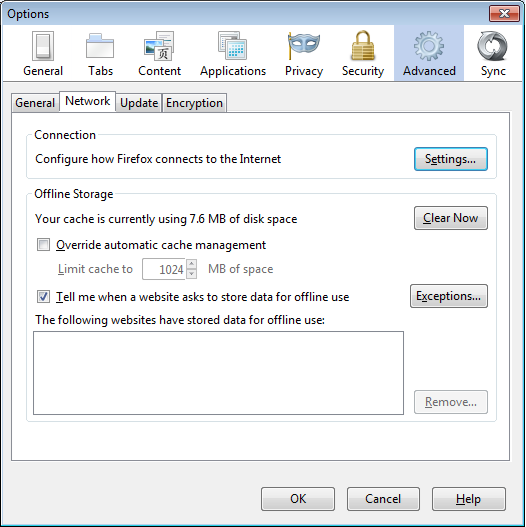
\includegraphics{ff_proxy_1.png}
\caption{Firefox Proxy Settings}
\end{figure}

Select Settings, click on ``Manual proxy configuration'' and enter the
information of the proxy server you want to use. Please remember that
HTTP proxies and SOCKS proxies work differently and have to be entered
in the corresponding fields. If there is a colon (:) in your proxy
information, that is the separator between the proxy address and the
port number. Your screen should look like this:

\begin{figure}[htbp]
\centering
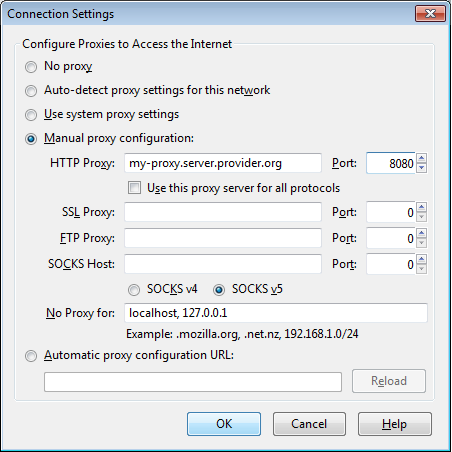
\includegraphics{ff_proxy_2.png}
\caption{Firefox Proxy Settings}
\end{figure}

After you click OK, your configuration will be saved and your Web
browser will automatically connect through that proxy on all future
connections. If you get an error message such as, ``The proxy server is
refusing connections'' or ``Unable to find the proxy server'', there is
a problem with your proxy configuration. In that case, repeat the steps
above and select ``No proxy'' in the last screen to deactivate the
proxy.
